\documentclass[a4paper]{article}

\usepackage{geometry}
\usepackage{natbib}
\bibpunct[:]{(}{)}{,}{a}{}{;}

%--------------------
%\usepackage{gb4e}
%\noautomath

\usepackage{amsmath}
\usepackage{amsfonts}
\usepackage{amsthm}
\usepackage{amssymb}
\usepackage{mathrsfs}
\usepackage{nicefrac}
%\usepackage{stmaryrd}
%\usepackage{multicol}
\usepackage{graphicx}
\usepackage{color}
\usepackage{booktabs}
%\newcommand{\mvalueof}[1]{\llbracket#1\rrbracket}
\newcommand{\citeposs}[2][]{\citeauthor{#2}'s (\citeyear[#1]{#2})}
\newcommand{\tuple}[1]{\ensuremath{\left\langle #1 \right\rangle}} 

\newcommand{\hl}[1]{\textcolor[rgb]{.8,.33,.0}{#1}}% prints in orange
%\newcommand{\argmax}[1]{\underset{#1}{\operatorname{arg}\,\operatorname{max}}\;}
%\newcommand{\argmin}[1]{\underset{#1}{\operatorname{arg}\,\operatorname{min}}\;}
%\newcommand{\sbna}{\exists\lnot\forall}

\definecolor{Red}{RGB}{178,34,34}
\newcommand{\mf}[1]{\textcolor{Red}{[mf: #1]}} 

%--------------------
%
%\usepackage{setspace}
%\onehalfspacing
%
%-------------------


\title{Tracing the cultural evolution of meaning at the semantics-pragmatics interface}

\author{%\bf NAME1 and NAME2\\
    ( -- draft \today --- )
}


\date{}

\begin{document}
\maketitle

\begin{abstract}
  According to standard linguistic theory, the meaning of an utterance is the product of a
  conventional semantic meaning of the used expression and general pragmatic reasoning applied
  to the context of utterance. This implies that models of the cultural evolution of meaning
  should likewise take into consideration that observable language use is a complex interaction
  of semantic representations and pragmatic use. To this end, we present a game theoretic model
  of the cultural evolution of language where communicative pressures work on abstract semantic
  representations and pragmatic patterns of use. Our model traces two evolutionary forces and
  their interaction: (i) fitness-based pressure towards communicative efficiency and (ii)
  systematic transmission perturbations when linguistic knowledge is transferred from one agent
  to another. The latter can arise from general cognitive or learning biases, but also from
  other sources of systematic noise, e.g., as a result of errors in perception. We illustrate
  the model based on a case study showing that cognitive biases that favor simple semantic
  representations can prevent the lexicalization of pragmatic inferences. We also show that,
  technically speaking, it is possible that environmental factors, such as perceptual errors
  during acquisition, can produce evolutionary outcomes that look as if such cognitive biases
  are present even if they are not.
\end{abstract}

\section{Introduction}\label{sec:introduction}
What is conveyed usually goes beyond what is said. A request for a blanket can be politely
veiled by uttering ``I'm cold.'' The temporal succession of events can be communicated by the
order in which conjuncts appear as in ``I traveled to Paris and got married.'' An invitation
can be declined by saying ``I have to work.'' An influential explanation of the relation
between the literal meaning of expressions and what they are intended and interpreted to convey
is due to \citet{grice:1975}. It characterizes pragmatic use and interpretation as a process of
mutual reasoning about rational language use. For instance, under the assumption that the
speaker is cooperative and relevant, ``I have to work'' may be interpreted as providing a
reason why the speaker will not be able to accept the invitation, going beyond its literal
meaning. Some of these enrichments are rather \emph{ad hoc}. Others show a striking
regularities, such as the use of questions for polite requests, or certain enrichments of
lexical meanings such as \emph{and} to mean \emph{and then}.

A particularly productive and well studied class of pragmatic enrichments are scalar
implicatures
\citep{horn:1984,Hirschberg1985:A-Theory-of-Sca,LevinsonPragmatics1983,Geurts2010:Quantity-Implic}. Usually,
an utterance of a sentence like ``I own some of Johnny Cash's albums'' will be taken to mean
that the speaker does not own all of them. This is because, if the speaker had them all, he
could have used the stronger word \emph{all} instead of \emph{some} in his utterance and
thereby would have made a more informative statement. Scalar implicatures, especially the
inference from \emph{some} to \emph{some but not all}, have been studied extensively, both
theoretically
\citep[e.g.][]{Sauerland2004:Scalar-Implicat,ChierchiaFox2008:The-Grammatical,Rooyvan-RooijJagerde-Jager2012:Explaining-Quan}
as well as experimentally
\citep[e.g.][]{BottNoveck2004:Some-Utterances,huang+snedeker:2009,GrodnerKlein2010:Some-and-Possib,GoodmanStuhlmuller2013:Knowledge-and-I,DegenTanenhaus2012:Processing-Scal}. While
there is much dispute in this domain and many interesting details, a position endorsed by a
clear majority is that a word like \emph{some} is underspecified to mean \emph{some and maybe
  all} and that the enrichment to \emph{some but not all} is part of some regular enrichment
process with roots in pragmatics.

If this majority view of underspecified lexical meaning and pragmatic enrichment routines is
correct, the question arises how such a system could have emerged in language evolution. Models
of meaning evolution abound. There are simulation-based models studying the evolution of
meaning in populations of communicating agents
\citep{Hurford1989:Biological-Evol,Steels1995:A-Self-Organizi,LenaertsJansen2005:The-Evolutionar,SteelsBelpaeme2005:Coordinating-Pe,BaronchelliPuglisi2008:Cultural-route-,steels:2011,SpikeStadler2016:Minimal-Require}
and there are mathematical models meaning evolution, mostly rooted in game theory
\citep{lewis:1969,Warneryd1993:Cheap-Talk-Coor,BlumeKim1993:Evolutionary-St,nowak+krakauer:1999,Huttegger2007:Evolution-and-t,Skyrms2010:Signals}. Much
work has focused on explaining basic properties such as compositionality and combinatoriality
\citep[e.g.][]{Batali1998:Computational-S,nowak+krakauer:1999,nowak+etal:2000,KirbyHurford2002:The-Emergence-o,kirby:2002,SmithKirby2003:Iterated-Learni,Gong2007:Language-Evolut,kirby+etal:2015,verhoef+etal:2014,Franke2015:Proto-Syntax}. But
little attention has been paid to the interaction between conventional meaning and pragmatic
use. 

To fill this gap, we here spell out a model of the co-evolution of conventional meaning and
pragmatic reasoning types. In other words, the object of evolutionary selection are pairs of
lexical meanings and general types of pragmatic behavior. Our model combines state-of-the-art
probabilistic cognitive models of pragmatic language use
\citep{frank+goodman:2012,FrankeJager2015:Probabilistic-p,GoodmanFrank2016:Pragmatic-Langu}
with a general and established model of language evolution
\citep{Hofbauer1985:The-Selection-M,nowak+etal:2000,NowakKomarova2001:Evolution-of-Un,Nowak2006:Evolutionary-Dy}. The
latter allows us to study the interaction between (i) evolutionary pressure towards
communicative efficiency and (ii) possible infidelity in the transmission of linguistic
knowledge, such as from inductive learning biases or systematic perceptual errors. This model
contains the most versatile dynamic from evolutionary game theory, the replicator dynamic
\citep{TaylorJonker1978:Evolutionary-St}, and a well-understood model of iterated Bayesian
learning \citep{griffiths+kalish:2007} as two special cases. The latter is particularly
important because in language learning agents need to infer unobservable conventional meanings
and pragmatic reasoning types from observable language use of their parent
generation. Section~\ref{sec:model} introduces this model.

Section~\ref{sec:si-case-study} applies this model to a case study on scalar implicatures. We
demonstrate a setting in which the majority view of underspecified lexical meanings and
pragmatic enrichments emerges, but only if selection and transmission infidelity are
combined. In particular, we show that inductive learning biases of Bayesian learners that favor
simpler lexical meanings can lead to the desired outcome. Additionally, we show how systematic
disturbances from environmental factors can lead to outcomes akin to those predicted under the
assumption of inductive learning biases. That is, that the regularization standardly predicted
to follow from learning biases can also emerge as a byproduct of noise.

% We see the main contribution of this work as conceptual and technical, not as a definite answer
% to the question why scalar implicatures emerged. The work here rather demonstrates how current
% probabilistic cognitive modeling of language use and evolutionary modeling can be fruitfully
% combined to study the co-evolution of semantics and pragmatics side-by-side.

\mf{on cultural evolution: \citet{Pagel2009:Human-Language-}}

\section{Model}
\label{sec:model}



\subsection{Communicative pressures at the semantics-pragmatics interface}
The emergence and change of linguistic structure is influenced by many intertwined factors. These range from biological and socio-ecological to cultural ones \citep{steels:2011}. Social and ecological pressures determine communicative needs, while biology determines the architecture that enables and constrains the means by which they can be fulfilled. In the following, our focus lies on the cultural aspects, wherein processes of linguistic change are viewed as shaped by language use and its transmission, i.e., as a result of a process of cultural evolution. 

The idea that language is influenced by communicative pressures has played a pivotal role in synchronic and diachronic analyses at latest since \citeposs{zipf:1949} rationalization of the approximation of word frequency rankings by a power law distribution as competing hearer and speaker preferences (e.g. in \citealt{martinet:1962, horn:1984,jaeger+vRooij:2007,jaeger:2007, piantadosi:2014,kirby+etal:2015}). In recent years, this line of research has led to a surge of approaches that seek to analyze the effects of such pressures from a multidisciplinary perspective, ranging from simulations to experiments with human and robotic agents (see \citealt{steels:2015} and \citealt{tamariz+kirby:2016} for recent overviews). Our starting point is given by the overarching argument that has crystalized from this literature: Natural languages need to be well-adapted to communicative needs within a linguistic community, but also need to be learnable to survive their faithful transmission across generations. More succinctly; natural languages are pressured for expressivity and learnability.   

The opposition of expressivity and learnability becomes particularly clear when considering their consequences in the extreme (cf. \citealt{kemp+regier:2012,kirby+etal:2015}). A language with a single form-meaning association is easy to learn but lacking in expressivity. Conversely, a language that associates a distinct form with all possible meanings a speaker may want to convey is maximally expressive but challenging to acquire. The most prominent problem that arises from this tension is that of acquiring a language to express a potentially infinite set of meanings through finite means \citep{kirby:2002}. However, this is not the only challenge learners confront. More central to our explanandum is the issue of selecting particular hypotheses out of a potentially infinite space of alternatives compatible with the data learners are exposed to. At the semantics-pragmatics interface this concerns the selection between functional (near-)equivalents, noting in particular that what is systematically conveyed through pragmatics could alternatively be codified lexically. Notwithstanding, lexical meanings that allow for pragmatic modifications often seem to resist the lexicalization of their pragmatic component. The question is why.

We assume an integral part of the answer to lie in the effects of transmission perturbations that arise when linguistic knowledge is acquired by new learners. As shown in the following, such perturbations may take the form of learning biases, but may also stem from extraneous factors such as a noisy perception of the environment.


We model these components using the replicator-mutator dynamics, combining functional pressure on successful communication with effects of transmission perturbations on (iterated) Bayesian learning \citep{griffiths+kalish:2007}. The semantics-pragmatics distinction and its bearing on production and comprehension are captured by a probabilistic model of rational language use with different degrees of pragmatic sophisitication and different lexica \citep{frank+goodman:2012,franke+jaeger:2014, bergen+etal:2016}. The remainder of this section introduces these components together with the assumptions underlying them. These are: the representation of languages and their use (\S\ref{sec:languages+use}), as well as pressures towards expressivity (\S\ref{sec:expressivity}) and learnability (\S\ref{sec:learnability}). After laying out the model, we analyze its predictions in a case-study on the lack of lexicalization of scalar implicatures in \S\ref{sec:si-case-study}. Additionally, \S\ref{subsec:noise} shows how the outcome predicted under the assumption of an inductive bias for simplicity in \S\ref{subsec:bias} can also arise from as a byproduct of the noisy perception of language users and learners. Section \S\ref{sec:discussion} discusses the general predictions of the model, as well as the implications drawn from its noisy counterpart.




\subsection{Lexica and linguistic behavior}\label{sec:languages+use}
Lexica codify the truth-conditions of a language's expressions. Following \citet{franke+jaeger:2014}, a convenient way to represent lexica is by $(|S|,|M|)$-Boolean matrices, where $S$ is a set of states of affairs (meanings) and $M$ a set of messages (forms available in the language).

We distinguish between two kinds of linguistic behavior. {\em Literal interlocutors} produce and interpret messages literally, being guided only by their lexica. {\em Pragmatic interlocutors} instead engage in mutual reasoning to inform their choices. Following models of rational language use such as Rational Speech Act models \citep{frank+goodman:2012} and their game-theoretic predecessors, the Iterated Best/Quantal Response models \citep{franke:2009,franke+jaeger:2014}, these behaviors are captured by a reasoning hierarchy. The hierarchy's bottom, level $0$, corresponds to literal language use. Pragmatic language users of level $n + 1$ behave rationally according to expected level $n$ behavior of their interlocutors. (\ref{h:level0}) and (\ref{h:leveln}) specify the behavior of literal and pragmatic hearers of a language $L$. Their speaker counterparts are given in (\ref{s:level0}) and (\ref{s:leveln}).

\begin{flalign}
&H_{0}(s|m;L) \propto pr(s) L_{sm} \label{h:level0}\\
&S_{0}(m|s;L) \propto \exp((L_{sm})^\alpha) \label{s:level0}\\
&H_{n+1}(s|m;L) \propto pr(s) S_{n}(m|s;L) \label{h:leveln}\\
&S_{n+1}(m|s;L) \propto  \exp(\lambda \; H_{n}(s|m;L)^\alpha) \label{s:leveln}
\end{flalign}


According to (\ref{h:level0}), a literal hearer's interpretation of a message $m$ as a state $s$ depends on her lexicon and her prior over states, $pr \in \Delta(S)$. For simplicity, in the following this prior is assumed to be uniform across hearers. The behavior of literal speakers, given in (\ref{s:level0}), is regulated by a parameter $\alpha$ which controls the sensitivity to which speakers prefer one signal over another based on its expected communicative success. 

Pragmatic behavior is similar to its literal counterparts. Their difference lies in that level $n+1$ speakers/hearers reason about level $n$ hearer/speaker behavior instead of solely relaying on their lexicon. That is, they reason about the way a rational level $n$ interlocutor would use or interpret a message, and behave according to these expectations.  Speaker behavior is further influenced by a soft-max parameter $\lambda$, $\lambda \geq 1$ \citep{luce:1959,sutton+barto:1998}. As $\lambda$ increases, choices made in production are more rational in that higher values lead to behavior that is increasingly in line with expected utility maximization. 

We call the combination of a lexicon with its use, i.e., a level in the reasoning hierarchy, a {\em type}. These are the basic units on which the model's dynamics operate. 

\subsection{Expressivity}\label{sec:expressivity}
Expressivity has received particular attention from investigations using evolutionary game theory (e.g. \citealt{nowak+krakauer:1999,nowak+etal:2000, nowak+etal:2002}). Under this view, a type's ability to convey and interpret information successfully confers it a higher fitness, a measure that is relative to the success of other types in the population. In the simplest models, fitness directly translates into the proportion of types present in the population after a generational turnover. This association of communicative success within a population with changes in the proportion of types present in it creates a feedback loop that pressures the population towards greater expressivity. 

The replicator equation gives us the means to make these dynamics precise. The proportion of types in a given population is codified in a vector $x$, where $x_i$ is type $i$'s proportion. As noted above, the fitness of type $i$ is equal to its relative communicative success within this population, $f_i = \sum_j x_j \text{EU}(t_i,t_j)$. The expected communicative success of $i$ and $j$ is simply the average success of $i$ conveying information to $j$ and vice versa: $\text{EU}(t_i,t_j) = [U_S(t_i,t_j) + U_R(t_i,t_j)]/2$. $U_S(x,y)$ and $U_R(x,y)$ are, respectively, $\sum_s P(s)\sum_m S_n(m|s;L) \sum_{s'} R_o(s'|m;L) \delta(s,s')$ and $U_S(y,x)$, for $n$ and $o$ being the reasoning level of $x$ and $y$, and $\delta(s,s') = 1$ iff $s = s'$ and $0$ otherwise. This quantity is symmetric, reflecting the probability of two types' mutual understanding. The average fitness of the population is given by $\Phi$, $\Phi = \sum_i x_i f_i$, serving as a normalizing constant for the discrete replicator equation: $\dot{x}_i = \frac{x_i f_i}{\Phi}$ 

Under its biological interpretation, the replicator dynamics capture the idea of fitness-relative selection whereby fitter types produce more offspring, leading to their propagation in subsequent generations. Many aspects of language are subject to transmission and change that can be likened to such biological processes. Amongst others, replication can be construed as modelling language acquisition, as e.g. in \citealt{nowak+etal:2002}, but also as a process of horizontal adaptation in a single generation (see \citealt[\S3.3]{benz+etal:2005b} for discussion).

In their series of papers on language evolution, Nowak and colleagues did not only consider expressivity but also recognized the central role of the fidelity by which language is transmitted. Among others, linguistic production can be prone to errors, states or messages may be percieved incorrectly, and multiple languages may be compatible with the data learners are exposed to. These sources of uncertainty introduce variation in their transmission from one generation to the next which can be likened to mutation to the effect that a type's offspring may adopt a different type than that of its parent as a result of transmission perturbations. Importantly, this variation should be relative to the learnability of a type under these perturbations (instead of, e.g., being a constant that is equal across all types as in \citealt{nowak+etal:2002}). For this purpose, we turn to a different strand of research in cultural evolution: iterated learning. 

%errors were considered in N+K:1999, mutation in N+etal:2002

\subsection{Learnability}\label{sec:learnability}
Iterated learning is a process in which the behavior of one individual serves as learning input for another. This learner, upon acquisition of this behavior, then goes on to produce behavior that serves as input for a new learner. This process can be thought of as a progression through chains of parents and children; the parent produces linguistic data from which the child infers a language. The latter, now a parent, goes on to produce data for a new generation of learners. Following \citet{griffiths+kalish:2007} we model iterated learning as a repeated process of Bayesian inference in which learners combine the likelihood of a type producing the received learning input with prior inductive biases. 

Due to the pressure towards learnability it exherts, iterated learning generally leads to simpler and more regular languages (see \citealt{kirby+etal:2014} and \citealt{tamariz+kirby:2016} for recent surveys). Importantly, experimental and mathematical results have been taken to suggest that the outcome of this process reflects learners' inductive biases. In a Bayesian setting these biases can be codified in a prior $P \in \Delta(T)$, which can be thought of as the amount of data a learner would require in order to adopt a language (cf. \citealt[450]{griffiths+kalish:2007}). Or, in our case, a combination of a lexicon and its use. The extent of the prior's influence has been shown to heavily depend on the learning strategy assumed to underly the inference process. On the one hand, early simulation results suggested that weak biases could be magnified by exposing learners to only small data samples (e.g. in \citealt{brighton:2002}). On the other, \citeposs{griffiths+kalish:2007} mathematical characterization showed that iterated learning converged to the prior, i.e., the resulting distribution over languages corresponds to the learners' prior distribution and is not influenced by the amount of input given to them. This difference in predictions can be traced back to differences in the selection of hypotheses from the posterior. Griffith \& Kalish's convergence to the prior holds for learners that sample from the posterior. More deterministic strategies such as the adoption of the type with the highest posterior probability, so-called {\it maximum a posterior estimation} (MAP), increase the influence of both the prior and the data \citep{griffiths+kalish:2007,kirby+etal:2007}. In the following, we parametrize the posterior by $l \geq 1$. In doing so, we obtain a range of learning strategies between posterior sampling and MAP. When $l = 1$ learners sample from the posterior and the learners propensity to maximize the posterior grows as $l$ increases.


The data learners are exposed to is described by a set $D$ containing sequences of state-message pairs, e.g., $\tuple{\tuple{s_i,m_v},...\tuple{s_j,m_w}}$. These are sequences of language use witnessed by learners, the length of which we denote by $k$. %Put differently, each datum $d \in D$ contains $k$ members of the set $\{\tuple{s_i,m_v} | s_i \in S, m_v \in M\}$.

%To summarize, the parametrized posterior, $P(d|t)^l$, is obtained from combining the prior $P(t)$ and the likelihood $P(d|t)$. Since types are combinations of a lexicon and its use, the latter can be computed straightforwardly from a type's production behavior. 
We combine the above with the replicator dynamics by codifying iterated learning in a transition matrix $Q$, where $Q_{ij}$ indicates the probability that a child of a parent of type $i$ adopts type $j$. This quantity is proportional to the probability of $i$ producing the learning data and that of inferring $j$ given the data: 


\[
 Q_{ij} \propto \sum_{d \in D} P(d|t_i) F(t_j,d), \; \text{where } F(t_j,d) \propto P(t_j|d)^l \text{ and } P(t_j|d) \propto P(t_j) P(d|t_j).
\]

\subsection{Model summary}
Drawing from past research, we argued that expressivity and learnability are central to the cultural evolution of language. We propose these components to be modelled respectively as communicative efficiency-relative replication and (iterated) Bayesian learning. Taken together their interaction is described by the replicator-mutator dynamics \citep{hofbauer+sigmund:2003}: 

\[ 
\hat{x}_i = \sum_j Q_{ji} \frac{x_jf_j}{\Phi}
\]

The units that the dynamics operate on are a combination of a lexicon and a degree of pragmatic sophistication determining its use. We call this combination a type. A type's expressivity depends on its communicative efficiency within a population while its learnability depends on the fidelity by which it is inferred by new generations of learners. The learners' task is consequently to perform a joint inference over types of linguistic behavior and lexical meaning. With this model at hand we turn to the analysis of the lack of lexicalization of productive pragmatic inferences in a case study on scalar implicatures. 


\section{Scalar implicatures}\label{sec:si-case-study}
%
Scalar implicatures are a particularly well-studied type of conventional pragmatic inferences. They are licensed for groups of expressions ordered in terms of informativity, here understood as an entailment induced order. For instance, {\em some} is entailed by {\em all}. If it were true that `All students came to class', it would also be true that `Some students came to class'. However, while weaker expressions such as {\em some} are truth-conditionally compatible with stronger alternatives such as {\em all}, this is not what their use is normally taken to convey. Instead, the use of a less informative expression when a more informative one could have been used can license a defeasible inference that stronger alternatives do not hold (cf. \citealt{horn:1972,gazdar:1979}). That is, a hearer who assumes the speaker to be able and willing to provide all relevant information can infer that stronger alternatives do not hold because the speaker used a weaker alternative instead. In this way, `Some students came to class' is strengthened to convey that some but not all students came to class. A bound that rules out stronger alternatives is thusly not codified in the lexical meaning of weak alternatives but instead pragmatically supplied.

This kind of strengthening is captured by the linguistic behavior of pragmatic types introduced in \S\ref{sec:languages+use}: A pragmatic hearer who reasons about a speaker's use of a message involving a weak scalar alternative will associate it more strongly with upper-bounded states than with ones in which stronger alternatives hold because these alternatives already unambiguously convey the latter states. Conversely, a pragmatic speaker will reason about her interlocutor's expected interpretation and use the messages at her disposition accordingly. 

Our initial question can now be narrowed to the case of scalar implicatures by asking for a justification for the lack of lexical upper-bounds in weak scalar alternatives. That is, why they are regularly selected for over other alternatives such as that of codifying the bound semantically. More poignantly, would it not serve language users better if weak(er) expressions such as {\em warm}, {\em or}, {\em some} and {\em big} were truth-conditionally incompatible with stronger alternatives such as {\em hot}, {\em and}, {\em all} and {\em huge}?  This question is particularly striking considering the number of expressions that license such inferences across languages. 

We see two main explanations for the lack of upper-bounds in the lexical meaning of weak scalar expressions. The first is that their truth-conditional compatibility with stronger expressions endows them with a broader range of applicability by allowing them to occur in contexts in which their upper-bounded reading is absent. This can happen when embedded in downward-entailing contexts, when the speaker is likely uncertain about whether the upper bounded reading is true, or when the distinction between an upper-bounded reading and the simple, only lower-bounded reading, is not relevant. For instance, if for all the speaker knows `Some students came' but she doesn't know whether all came, then the use of {\em some} lacking an upper-bound succinctly conveys her uncertainty. This may suggest a functionalist argument for why upper-bounded meanings do not conventionalize: Should contextual cues provide enough information to the hearer to identify whether a bound is intended to be conveyed pragmatically, then this is preferred over expressing it overtly through longer expressions, e.g., by saying {\em some but not all} explicitly. Importantly, although morphosyntactic disambiguation may be dispreferred due to its relative length and complexity \citep{piantadosi+etal:2012b}, it allows speakers to enforce an upper-bound and override contextual cues that might otherwise mislead the hearer. In a nutshell, this explanation posits that scalar implicatures fail to lexicalize because, all else being equal, speakers prefer to communicate as economically as possible and pragmatic reasoning enables them to do so. Compare this with a hypothetical language that lexicalizes two expressions for each weak scalar expression -- one with and one lacking an upper-bound. We see four conditions along this functionalist explanation that may pressure languages for English-like semantics over this alternative. First, contextual cues are very reliable. Second, morphosyntactic disambiguation is seldom necessary. Third, morphosyntactic disambiguation is only marginally dispreferred. Fourth, larger lexica are costly. Overall, neither condition seems convincing as a pivotal explanatory device for such a widespread phenomenon. The first two conditions put a heavy burden on the ability to retrieve contextual cues to a degree that seems unlikely to undercut the benefit of unambiguous communication. It is likely that human language users are very good at retrieving cues from context, but to stipulate that they are so good as to undercut the benefit of safe communication provided by this hypothetical alternative strikes us as too strong of an assumption.  As for the third and fourth condition, these seem mostly like technical solutions without a proper empirical basis. 

Instead, the systematicity and typological spread of scalar implicatures together with the observation that monomorphemic expressions that lexically rule out stronger alternatives are unattested across languages (\citealt[252-267]{horn:1984}, \citealt{horn:1972,traugott:2004,vdAuwera:2010}) suggests that other forces may be at play. In what follows we investigate the hypothesis that the lack of lexicalization of scalar inferences may be accounted for by the relative representational simplicity of lexical meanings lacking an upper-bound over those that explicitly codify it. This difference is reflected in a learning bias towards more compressed lexical representation, i.e., in a preference of learners for simpler over more complex explanations of the data they witness \citep{feldman:2000, chater+vitanyi:2003, piantadosi+etal:2012a, kirby+etal:2015,piantadosi+etal:underreview}. 

While we do not want to argue that functional aspects as the ones discussed above do not play a role, we do see a clear benefit in exploring whether matters of transmission biases would not give us additional explanatory leverage. Note however that we do not represent the contrast between lexical representations explicitly. Instead, the bias is directly encoded in the learners' prior over types. In principle this difference could be made precise with an adequate representational language, e.g., through measures over representational complexity such as minimal description length.  There is a growing effort to develop such empirically  testable  representational  languages. For  instance, the so-called {\em language of thought} has been put to test in various rational probabilistic models that show encouraging results (see e.g. \citealt{katz+etal:2008, piantadosi+etal:underreview, piantadosi+etal:2012a} and references therein). We think that our assumption is well-warranted as a working hypothesis and decide against such an enrichment at present in order to focus on the effects of linguistic pressures predicted the model instead.




\subsection{Analysis}
We analyze the model's predictions in populations of types with two signaling behaviors; literal and pragmatic. The former correspond to level $0$ reasoners who only take their lexica into consideration and the latter to level $1$ reasoners. Higher level reasoning is not required to derive scalar implicatures from the lexica we consider here, nor do they leave room for substantial pragmatic refinement.

The space of possible lexica is given in Table \ref{tab:lexica}. These $(2,2)$-Boolean matrices are the simplest ones that allow us to make the contrast between the presence or abscence of an upper-bound and the use of scalar implicatures precise. One may think of the state corresponding to the first row of any such lexicon as a ``some but not all''-state and the second as an ``all''-state. The literal meaning of weak scalar expressions such as English {\em some} then corresponds to a message true of both rows in these fragments. While there are $16$ possible $(2,2)$-lexica, a number of them are identical both in terms of expressivity and the learning bias. The competition between such types is determined by the initial configuration of a population. However, this can be obscured when averaging across simulations. We focus on this smaller representative subset as simulations conducted with the full space confirm that the general results reported here do not hinge on this choice.

Lexica $L_1$ to $L_3$ are not optimal for communication because they assign the same state to all their messages. This failure to be able to associate a single form to a state inevitably leads to a communicative disadvantage in their use. $L_4$ and $L_5$ are our target lexica. They codify upper-bounded semantics for the message corresponding to the first matrix's column and a lack thereof, respectively. Lastly, $L_6$ is similar to $L_5$ in that two messages are true of the same state but differs from it in assigning upper-bounded semantics to the first column's message. 

\begin{table}[t]
\centering 
\begin{tabular}{l c l}
$L_1$ = $\begin{pmatrix} 0 & 0 \\ 1 & 1 \end{pmatrix}$ & 
$L_2$ = $\begin{pmatrix} 1 & 1 \\ 0 & 0 \end{pmatrix}$ & 
$L_3$ = $\begin{pmatrix} 1 & 1 \\ 1 & 1 \end{pmatrix}$\\[0.5cm]

$L_4$ = $\begin{pmatrix} 1 & 0 \\ 0 & 1 \end{pmatrix}$ &
$L_5$ = $\begin{pmatrix} 1 & 0 \\ 1 & 1 \end{pmatrix}$ &
$L_6$ = $\begin{pmatrix} 1 & 1 \\ 0 & 1 \end{pmatrix}$
\end{tabular}
\caption{Space of possible lexica.}
\label{tab:lexica}
\end{table}




Combining a linguistic behavior with each of these $6$ lexica yields a total of $12$ distinct types. Note in particular  that a type that has conventionalized upper-bounds to realize a (quasi-)partition of the relevant semantic space, such as $L_4$, will produce speaker behavior that is {\em almost} indistinguishable from that of a language that lacks upper-bounds, but with pragmatic users, such as $L_5$. Almost, because there may be slight differences between the probability with which speakers would (erroneously) use a semantically false description and the probability with which speakers would (erroneously) use a pragmatically suboptimal description. Due to this possibly marginal difference between pragmatic $L_4$ and $L_5$, the selection of one type over the other is expected to mainly depend on their transmission to new learners. Things are less clear for literal $L_5$ contrasted with literal/pragmatic $L_4$ as the former has a learning advantage under the inductive bias but is expected to fare worse in communicative terms.


The dynamics are initialized with an arbitrary distribution over types, constituting the population's first generation. The results for each parameter setting were obtained from $1000$ independent runs, each consisting of $20$ generations. This corresponds to a developmental plateau after which no noteworthy change was registered. As specified in \S\ref{sec:learnability}, the learning matrix $Q$ can be obtained by considering all possible state-message sequences of length $k$. Given that this is intractable for large $k$, matrices were approximated by sampling $10$ sequences from each type's production probabilities and a type's children being exposed only to this subset. 

%For convenience, the model's parameters are summarized in Table \ref{tab:summary}.
%
%\begin{table}
%\centering
%\begin{tabular}{l|l|l}
%    \multicolumn{1}{c}{parameter} & \multicolumn{1}{c}{explanation} & \multicolumn{1}{c}{locus}\\ \hline
%    $\lambda \geq 1$ & rationality parameter & $S_{n+1}(m|s;L) \propto \text{exp}(\lambda \; H_{n}(s|m;L)^\alpha)$\\
%    $\alpha \in [0,1)$ & semantics-pragmatics tension & $S_{n+1}(m|s;L) \propto \text{exp}(\lambda \; H_{n}(s|m;L)^\alpha)$\\ 
%    $|D|$ & number of data produced per parent type & $P(d|t_j)P(t_i|d)$\\
%    $k = |d|$ & number of observations per datum& $P(d|t_j)P(t_i|d)$\\
%    $l \geq 1$ & posterior parameter from sampling to MAP & $P(t_i|d) \propto [P(t_i)P(d|t_i)]^l$\\
%    $c \in [0,1]$ & learning bias for lack of upper-bounds &  $P(t_i)$
%\end{tabular}
%\caption{Summary of model parameters.} 
%\label{tab:summary}
%\end{table}
\subsection{Transmission bias}\label{subsec:bias}
Following our assumption of a preference for simple lexical representations, the prior biases learners against lexica in which a message holds true only of the first row, i.e., against messages that lexicalize an upper-bound that rules out the ``all''-state. All other semantics are assumed to be a priori equally probable. This is captured by $P(t_i) \propto n - c \cdot r$, where $n$ is the total number of states and $r$ is the number of messages only true of row $1$ in $t_i$'s lexicon, $c \in [0,1]$. Increments in the value of $c$ therefore bring about a stronger bias against languages that lexicalize upper-bounds, i.e., $L_2, L_4$ and $L_6$.

According to our hypothesis, functional pressure on successful communication combined with learning pressures in the form of a bias against upper-bounds may lead to the selection of $L_5$-like semantics. It is instructive to first inspect the effect of these pressures in isolation. For this purpose we focus our attention on three pragmatic types.\footnote{Pragmatic reasoning allows language users to refine their (possibly erroneous) choices. Therefore, it is advantageous even for those types that codify an upper-bound lexically.} Pragmatic $L_3$, a type that is lacking in expressivity but is a priori preferred for its lack of upper-bounds. Pragmatic $L_4$, a type that is functionally advantageous but biased against. And pragmatic $L_5$, combining virtues of the latter two.  

\paragraph{Expressivity only.} The replicator dynamics are sensitive to $\lambda$ and $\alpha$ as both have a bearing on a type's fitness. The influence of the rationality parameter for is depicted in Figure \ref{fig:either-R-or-M}.A. The less expressive $L_3$ speakers fare the worse and are influenced the least by change in $\lambda$. In contrast, low values of $\lambda$ result in a higher proportion of $L_4$ speakers relative to $L_5$. This is expected given role of rationality in producing more deterministic behavior in users of $L_5$-like languages. As the rationality parameter increases, the functional difference between $L_4$ and $L_5$ is leveled. Overall, the outcome from only a pressure towards expressivity approximates an even share of pragmatic $L_4, L_5$ and $L_6$ types. The latter follows the same trajectory as $L_5$ in Figure \ref{fig:either-R-or-M}.A.  This illustrates the problem we started out with: expressivity alone can not differentiate between (near-)functional equivalents to a degree that justifies the systematic prevalence of $L_5$-like semantics.  


%In particular, low $\alpha$ disadvantages types that rely on pragmatic reasoning to the gain of those that codify more semantically. The rationality parameter $\lambda$ has a similar effect for different reasons: Low rationality leads to a less pronounced preference for the choice(s) expected to succeed best in communication. That is, $\lambda$ regulates the strength by which users of $L_5$ associate non-upper-bounded $m_1$ exclusively with the ``some''-state $s_1$ over the ``all''-state $s_2$. Speakers of $L_4$ need not rely on $\lambda$ for this as the association of $m_1$ with $s_1$ is already part of their language's semantics.


\begin{figure}
\centering
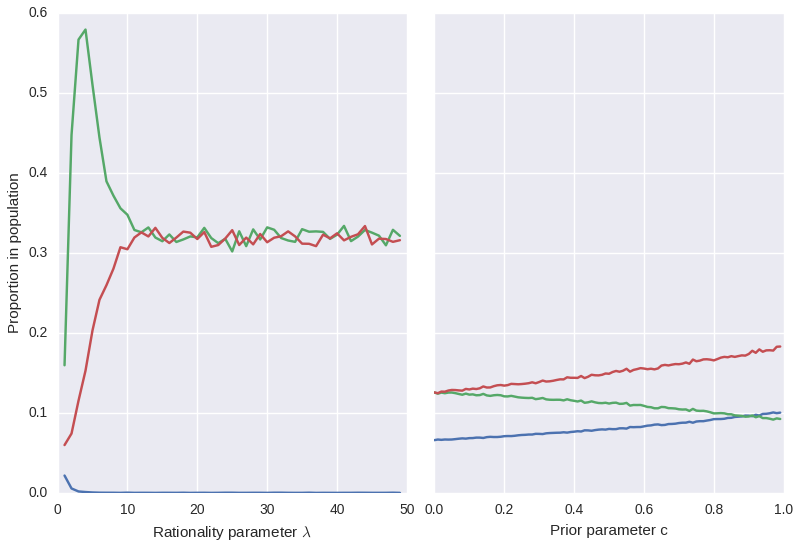
\includegraphics[scale=.5]{./only-R-or-M}
\caption{Mean proportions of target types after $20$ generations in $1000$ populations with only a pressure for expressivity in A ($\alpha = 1$) and only for learnability in B ($\alpha =1, \lambda = 30, k = 5$, $l=1$).}
\label{fig:either-R-or-M}
\end{figure}

\paragraph{Learnability only.} The effect of iterated learning with posterior sampling but without a pressure for expressivity is shown in Figure \ref{fig:either-R-or-M}.B. In line with our expectations, the share of $L_4$ speakers decreases as the bias against upper-bounds increases. In turn, this benefits $L_3$ and, in particular, $L_5$. However, even a strong bias against lexical upper-bounds leads only to a moderate advantage of $L_5$ over $L_4$. More importantly, a pressure only towards learnability can promote functionally defective languages such as $L_3$.

Inspecting these pressures separately not only showcases the influence of some model components but also highlights some of their broader implications. First and foremost, neither dynamic comes close to converging to a monomorphic population under most parameter configurations. For instance, while $L_4$ speakers can come to take over a substantial proportion of the population, this only happens in a restricted range of low degrees of rationality. Apart from polymorphy, both pressures make undesirable predictions when considered in isolation. A pressure only towards expressivity leads to the expulsion of communicatively suboptimal $L_1$, $L_2$ and $L_3$ from the population but can not explain the regular selection of $L_5$-like semantics over either of its functionally similar alternatives. A pressure only towards learnability has a modest but clear effect in differentiating $L_5$ from these alternatives but fails to rule out functionally suboptimal types such as tautological $L_3$. 

\begin{figure}
\centering
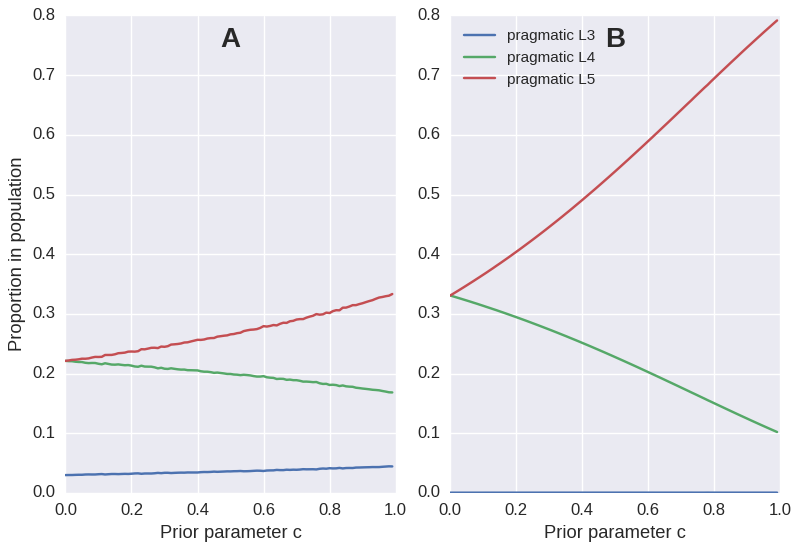
\includegraphics[scale=.5]{./fig2-rmd}
\caption{Mean proportions of target types after $20$ generations in $1000$ populations across bias values $c \in [0,1]$ with $l =1$ in A and $l = 3$ in B ($\alpha =1, \lambda = 20, k = 5$).}
\label{fig:cost}
\end{figure}

\paragraph{Expressivity and learnability.} Figure \ref{fig:cost} illustrates the effect of the learning bias for posterior sampling (\ref{fig:cost}.A) and slightly more MAP-like learning (\ref{fig:cost}.B) when pressured for both expressivity and learnability.\footnote{\hl{Robert suggests to illustrate the effect with a higher l-value. E.g., l = 1 and l = 10}} More detailed results for all types across a sample of $c$-values for $l = 1$ and $l = 3$ are presented in Table \ref{tab:numeric-results}. These results show that a weak bias is sufficient to lead to a selection of $L_5$ over $L_4$. As in the outcomes that only considered learnability, this effect increases with the bias' strength provided $L_5$ users are pragmatic. Importantly, the addition of a pressure towards expressivity magnifies this effect and dampens the proliferation of functionally suboptimal types advantaged by the learning bias. As stressed above, this indicates that neither a learning bias nor functional pressure alone but their combination may lead to the lack of upper-bounds in the lexical meaning of scalar expressions.


\begin{table}
\centering 
\begin{tabular}{l | c c c c c| c c c c c c c c}
\multicolumn{1}{c}{~} & \multicolumn{5}{c}{$l = 1$} & ~ & \multicolumn{5}{c}{$l = 3$}\\ \hline \hline
  c        &  0  & .1  & .5  & .8  & .9 & ~ & 0 & .1 & .5 & .8 & .9\\ \hline \hline
lit. $L_1$ & .03 & .03 & .04 & .04 & .04& ~ & 0 &0 & 0 & 0 & 0\\ 
lit. $L_2$ & .03 & .03 & .02 & .01 & .04& ~ & 0& 0 & 0 & 0 & 0\\
lit. $L_3$ & .03 & .03 & .04 & .04 & .04& ~ & 0& 0 & 0 & 0 & 0\\
lit. $L_4$ & .07 & .07 & .06 & .06 & .05& ~ & 0& 0 & 0 & 0 & 0\\
lit. $L_5$ & .04 & .05 & .05 & .06 & .06& ~ & 0& 0 & 0 & 0 & 0\\
lit. $L_6$ & .04 & .04 & .04 & .04 & .03& ~ & 0& 0 & 0 & 0 & 0\\ \hline
prg. $L_1$ & .03 & .03 & .04 & .04 & .04& ~ & 0& 0 & 0 & 0 & 0 \\
prg. $L_2$ & .03 & .03 & .02 & .01 & .04& ~ & 0& 0 & 0 & 0 & 0 \\
prg. $L_3$ & .03 & .03 & .04 & .04 & .04& ~ & 0& 0 & 0 & 0 & 0 \\ 
prg. $L_4$ & .22 & .22 & .2 & .18 & .17& ~ & .33& .31 & .23 & .15 & .12 \\
prg. $L_5$ & .22 & .23 & .27 & .3  & .32& ~ & .33& .37 & .54 & .7 & .75 \\
prg. $L_6$ & .22 & .22 & .2 & .18 & .17& ~ & .33& .31 & .23 & .15 & .12
\end{tabular}
\caption{Mean proportions of types in $1000$ populations after $20$ generations across bias values $c \in [0,1]$ with $l =1$ and $l = 3$ ($\alpha = 1, \lambda = 30, k = 5$)}%, $\epsilon < 0.005$.}
\label{tab:numeric-results}
\end{table}

Other than the consideration of both pressures, the resulting proportion of pragmatic $L_5$ speakers primarily hinges on three factors. First, the degree to which linguistic behavior is deterministic, as it plays a role both for expressivity as well as in producing data that allows learners to discriminate this type from others. Second, the inductive bias, which controls the learners preference for simpler lexical representations. Lastly, the posterior parameter, which magnifies the effects of the learning bias in tandem with replication. 

As discussed in relation to Figure \ref{fig:cost}.A, posterior sampling can lead to the incumbency of pragmatic $L_5$. However, not even a strong favorable learning bias combined with a pressure for expressivity completely drives out competing types. This is not so for more posterior maximizing behavior. As shown in Figure \ref{fig:prior-posterior}, the range of bias values within which $L_5$ takes over the population increases with MAP-like learning. In other words, the strength of the learning bias required for a given final proportion of $L_5$ speakers strongly depends on learners' inferential strategy. As for the effect of the other parameters not mentioned so far, changes in sequence length influence the population in a predictable way: smaller values lead to more heterogeneous populations that reflect the learner's prior more faithfully. Larger ones lead to more pronounced differences amongst equally preferred types. This is due to the fact that the likelihood that a small sequence was produced by any type is relatively uniform (modulo prior) compared to that of types with lexica $L_1$ - $L_3$ to produce larger sequences with the same state-message combination in contrast to pragmatic speakers of $L_4$ - $L_6$, or literal $L_4$.


\begin{figure}
\centering
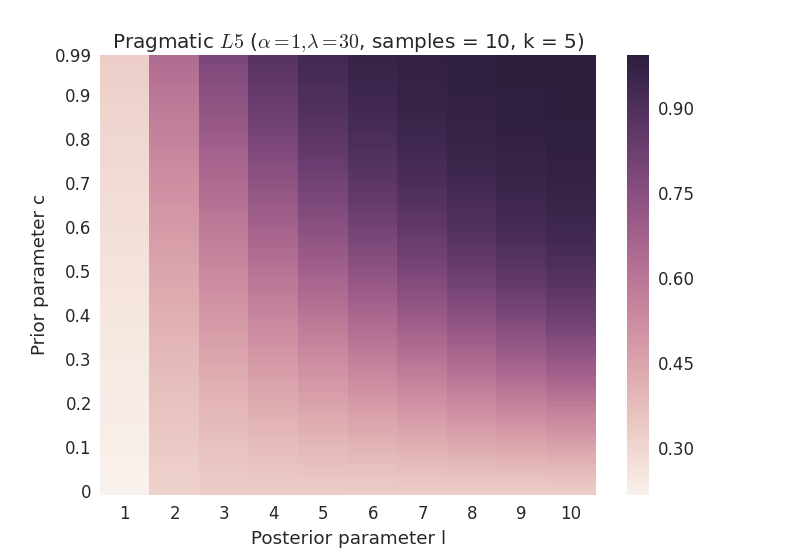
\includegraphics[scale=.5]{../presentations/01heatmap}
\caption{Mean proportion of pragmatic $L_5$ in $1000$ populations after $20$ generations ($\alpha = 1, \lambda = 30, k = 5$)}
\label{fig:prior-posterior}
\end{figure}


\subsection{Discussion}
Under the assumption of a learning bias for simpler representations, our results suggest that a lack of semantic upper-bounds coupled with pragmatic reasoning can overcome communicative pressures and stabilize in a population. This prediction hinges on three assumptions. First, that language is pressured toward both expressivity and learnability. Second, that language use is relatively deterministic -- low $\lambda$ renders languages that rely on pragmatics to associate one state to one message too prone to communicative failure and more difficult to learn. Lastly, that learners prefer simpler over more complex lexical representations. An important addendum to this third condition being that a combination of rationality in choice and maximization in learning requires a weaker bias towards simplicity. Under these conditions the selection of lexical meanings lacking upper-bounds in populations of pragmatic speakers is robust against parameter perturbations.  This outcome is particularly encouraging in light of other advantages a lack of semantic upper-bounds may confer. 

While non upper-bounded lexical meanings in weak scalar alternatives are predicted by the literature, it not clear to what extent other types should be present in the final population, if at all. It seems reasonable to expect functionally suboptimal types $L_1$, $L_2$ and $L_3$ to be ruled out because they fail to enable their users to communicate effectively. However, this is not true of $L_4$.\footnote{$L_6$ presents a special case. In our current setup, it mirrors $L_5$ in enabling for the pragmatic strengthening of a message that does not codify an upper-bound lexically. However, this is achieved by ruling out the ``some but not all''-state and not, as with scalar implicatures, the ``all''-state. $L_6$ speakers therefore strengthen a ``some''-message to convey something paraphrasable as `some but not [some but not all]'. The current representation of lexica as Boolean matrices is blind to this anomaly without further restrictions.} Notwithstanding, the prediction that natural language communities are homogeneous or that a single speaker may entertain $L_4$-like semantics for one scalar expression and $L_5$-like semantics for another is not implausible (cf. \citealt{franke+degen:2016}). Alternatively, a stronger tendency for posterior maximization has to be assumed (see Figure \ref{fig:prior-posterior}). This empirical issue relates to other two aspects left undiscussed: disadvantages of pragmatic reasoning and the effect of state frequencies on the fossilization of pragmatic inferences. We tacitly assumed pragmatic reasoning to come at no cost. However, there is experimental evidence that suggests  that the pragmatic derivation of upper-bounds costs effort and takes additional processing time (cf. \citealt{deNeys+schaeken:2007, huang+snedeker:2009}). This raises the question at which point such usage-based cost undercuts the learnability advantage of simpler semantic representations. Should cost play a role, then its effect is bound to depend on the frequency with which a given scalar expression is used. It is therefore plausible that frequently drawn scalar implicatures might fossilize to avoid cost, while infrequent ones could still be computed on-line. This opens a possible venue to address the first question about the expected presence of $L_4$-like semantics, but further empirical evidence is needed to assess these matters beyond speculation. 


\subsection{Noisy transmission}\label{subsec:noise}
The assumption of a learning bias was pivotal in introducing transmission perturbations that differentiate functionally similar types. However, these perturbations need not necessarily arise from inductive biases. As shown in the following, outcomes that are indistinguishable from the ones predicted above can come about through environmental factors such as perceptual errors during production and comprehension as well. We should stress that we do not want to suggest noisy perception to underlie the selection of a lack of semantic upper-bounds in scalar items. Instead, our goal is to stress the role that transmission perturbations play in this process and the cultural evolution of meaning more broadly, as well as to highlight the explanatory potential environmental forces, which have received less attention than their inductive counterparts.

The core components of the model remain as before. All that is required is their adjustment to the possibility of confusing one state with another by language users and learners. Letting $\epsilon$ stand for the probability of confusing the first row state with the second, and vice-versa for $\delta$, we denote the probability that the teacher (learner) observes state $s_t$ ($s_l$) when the actual state is $s_a$ as $P_N(s_t \mid s_a)$ ($P_N(s_l \mid s_a)$). The probability that $s_a$ is the actual state when the learner observes $s_l$ is therefore:

\begin{align*}
  P_N(s_a \mid s_l) \propto P(s_a) \ P_N(s_l \mid s_a)\,.
\end{align*}

Accordingly, the probability that the teacher observes $s_t$ when the learner observes $s_l$ is:
\begin{align*}
  P_N(s_t \mid s_l) = \sum_{s_a} P(s_a \mid s_l) \ P_N(s_t \mid s_a)\,.
\end{align*}
Finally, this gives us the probability that a teacher of type $t$ produces a datum that is
perceived by the listener as $d = \tuple{s_l, m}$:
\begin{align*}
  P_N(\tuple{s_l, m} \mid t) = \sum_{s_t} P_N(s_t \mid s_l) \ P(m \mid s_t; t)\,.
\end{align*}
Generalize this to a sequence of perceived data $d_l$ and write $P_N(d_l \mid t)$. Then, the noise-perturbed mutation matrix is defined as:
\begin{align*}
  Q_{ij}  \propto \sum_{d_l \in D} P(d_l \mid t_i) F(t_j,d_l) \,, \ \  \text{where $F(t_j,d)$
    is as before.}
\end{align*}
In words, it may be the case that learner and/or teacher do not perceive the actual state as what it is. They are not aware of this, and produce/learn as if what they observed was the actual state. In particular, the learner does not reason about noise when she tries to infer the speaker's type. She takes what she observes a state to be as the actual state that the teacher has seen as well and infers which type would have most likely generated the message to this state. This can lead to biases of inferring the ``wrong'' teacher type, if the noise makes some types err in a way that resembles the noiseless behavior of other types. That is, such environmental factors can, in principle, induce transmission biases that look as if there was a cognitive bias in favor of a particular type, simply because that type better explains the noise.

Apart from changing the mutation matrix in this way, we also need to adapt the calculation of expected utilities, taking into consideration that states are perceived noisily:
\begin{align*}
  U_S(t_i,t_j) = \sum_{s_a}  P(s_a) \sum_{s_t} P_N(s_t \mid s_a) \sum_m S_n(m|s_t;L) \sum_{s'} R_o(s'|m;L) \delta(s,s')\,.
\end{align*}


\paragraph{Results.} As shown in Table \ref{tab:num-noise}, a prevalence of pragmatic $L_5$ can also arise from noisy transmission without a learning bias for particular types $(c = 0)$. In contrast to the outcome predicted by its noiseless counterpart, favourable outcomes for this type concentrate in parameter configurations  with $\epsilon > \delta$, $\alpha \geq 5$, $1 < k < 20$ and $l > 3$. As stressed above, we are not concerned with the interpretation of these particular values for the case study at hand, but rather with the technical result that shows that the mere presence of systematic noise in the transmission of strategies can introduce regularization that looks as if the agents have a learning bias. In other words, learning biases are clearly not the only transmission perturbations that shape cultural evolution alongside functional pressure. Environmental and perceptual noise can play a role too.

\begin{table}
\centering 
\begin{tabular}{l | c c c c c| c c c c c c c c}
\multicolumn{1}{c}{~} & \multicolumn{5}{c}{$l = 5$} & ~ & \multicolumn{5}{c}{$l = 15$}\\ \hline \hline
 ($\epsilon,\delta$)        &  (.1,.1)  & (.1,.3)  & (.3,.1)  & (.8,.1)  & (.1,.8) & ~ & (.1,.1) & (.1,.3) & (.3,.1) & (.8,.1) & (.1,.8)\\ \hline \hline
lit. $L_1$ & .01 & .02 & .03 & .03 & .03& ~ & 0& .02&  .02 & .01 & .01\\ 
lit. $L_2$ & .01 & .02 & .03 & .03 & .03& ~ & 0& .02&  .02 & .01 & .01\\
lit. $L_3$ & .01 & .02 & .03 & .01 & .03& ~ & 0& .02 & .02 & .01 & .01\\
lit. $L_4$ & .03 & .03 & .03 & .05 & .01& ~ & .04& .03 & .03 & .01 & .01\\
lit. $L_5$ & .02 & .04 & .03 & .02 & .02& ~ & .01& .03 & .02 & .02 & .01\\
lit. $L_6$ & .02 & .03 & .04 & .03 & .05& ~ & .01& .03 & .04 & .01 & .02\\ \hline
prg. $L_1$ & .01 & .02 & .03 & .03 & .03& ~ & 0&  .02& .02 & .01 &  .01\\
prg. $L_2$ & .01 & .02 & .03 & .03 & .03& ~ & 0&  .02& .02& .01&  .01\\
prg. $L_3$ & .01 & .02 & .03 & .03 & .03& ~ & 0&  .02& .02 & .01 & .01 \\ 
prg. $L_4$ & .45 & .11 & .11 & .02 & .02& ~ & .44& .11 & .1 & .22 & .02 \\
prg. $L_5$ & .22 & .17 & .47 & .04 & .68& ~ & .24& .18 & .56 & .02 & .84\\
prg. $L_6$ & .22 & .48 & .17 & .69 & .04& ~ & .24& .52 & .16 & .84 & .02
\end{tabular}
\caption{\hl{Currently: Mean proportions of types from $50$ runs per $100$ independently generated Q-matrices per parameter setting after $20$ generations across noisy values for $\epsilon$ and $\delta$ with $l = 5$ and $l = 10$ ($\alpha = 10, \lambda = 20, k = 5$). In principle, we could skip every second row because pragmatic $L5$ and $L6$ mirror each other.}}
\label{tab:num-noise}
\end{table}



\section{General discussion}\label{sec:discussion}
We laid out a model that combines game theoretical models of functional pressure towards efficient communication \citep{nowak+krakauer:1999}, effects of transmission perturbations on (iterated) language learning \citep{griffiths+kalish:2007}, probabilistic speaker and listener types of varied degrees of pragmatic sophistication \citep{frank+goodman:2012, franke+jaeger:2014} as well as different lexica \citep{bergen+etal:2012,bergen+etal:2016}. This model generates predictions about lexicalization patterns and, more generally, effects of communicative pressures on the cultural evolution of language. We argued that the puzzle raised by semantics in light of pragmatics is hard to explain on purely functional grounds and that part of the answer may instead lie in the way transmission shapes the outcome of cultural evolution in tandem with a pressure for successful information transfer. In the realm of inductive biases, we adopted the assumption that simpler semantic representations are more likely to be learned (cf. \citealt{chater+vitanyi:2003}). Under this view, semantics and pragmatics play a synergic role in that representational simplicity is supplemented by pragmatic reasoning to counteract functional disadvantages otherwise incurred. As a consequence, iterated transmission and use of language lead to a regularization that may explain the lack of lexicalization of systematic pragmatic enrichments. This result is of particular relevance for the longstanding assumption of a divide and interaction between semantics and pragmatics by offering an account of why (certain) pragmatic inferences fail to lexicalize. More generally, we showed that systematic noise in perception can produce outcomes that are indistinguishable from those generated by inductive biases. This adds to \citeposs{franke+correia:toappear} argument that linguistic regularities may arise as a byproduct of noise, rather than through inductive biases.


The main innovations of the model are its modular separation of expressivity and learnability, allowing for their isolated and combined analysis, the learning process involving a joint inference over types of pragmatic behavior and lexical meaning, as well as in its accommodation of different transmission perturbations that go beyond learning biases. The goal to decouple but model both expressivity and learnability has also recently been addressed by \citet{kirby+etal:2015}. In contrast to our proposal, Kirby et al. model expressivity as exerting its force only in the production of learning data. This model's expressivity parameter thereby fulfills a similar role  to high values of $\lambda$ in making speaker behavior more deterministic. In this way, it ``favors'' unambiguous languages. However, the degree of mutual understanding of interlocutors central to replication and to our notion of expressivity is not taken into consideration. That is, while our proposal combines bidirectional horizontal transmission with its vertical and unidirectional counterpart, Kirby et al.'s model only considers the latter's influence. Our reasoning behind the inclusion of the former lies in the empirical and theoretical observation that learnability alone can lead the selection of functionally defective languages, as showcased by the tautological language $L_3$ in our analysis. This outcome has been reported in a number of laboratory experiments where the participants' task was to learn and subsequently reproduce the language produced by a previous participant, leading to a proliferation of languages that associated a large number of meanings with a single form (see e.g. \citealt{silvey+etal:2014} and experiment 1 in \citealt{kirby+etal:2008}). In contrast, experiments involving an interactive component have been found to foster languages that enable interlocutors to distinguish meanings accurately  (e.g. \citealt{fay+etal:2013}; for a review of laboratory results under the iterated learning paradigm and further discussion see \citealt{kirby+etal:2015, tamariz+kirby:2016}). It is not evident how to compare these findings given that they consider distinct meaning spaces, modes of transmission, iterations and feedback given to participants. However, we take these results to suggest that there is an important difference between a language generating learnable linguistic data and its actual performance as a means of information transfer. The former solely depends on the mechanism by which speakers associate form and meaning. The latter additionally hinges on the addressee's linguistic experience and her ability to interpret linguistic input based on this experience. In sum, we contend that successful information transfer in a linguistic community is central to the adoption of a communication system and that this measure is not adequately reflected by production alone.

The demonstration that noise can lead to regularized evolutionary outcomes that are indistinguishable from those generated by prior learning biases is relevant not for the case study at hand, but more so for the broader project of analyzes of the cultural evolution of language. On the one hand, the plurality of sources of transmission perturbations admitted by these models paints a cautionary tale for the design of studies that purport to provide explanatory accounts of linguistic phenomena. In particular, when the outcome is interpreted as informative about the perturbation assumed to generates it (cf. \citealt{tamariz+kirby:2016}). On the other, and most importantly, it showcases how regularities can arise as a byproduct of systematic noise rather than from standardly assumed inductive biases.



\section{Conclusion}
The cultural evolution of language is influenced by intertwined pressures. We set out to investigate this process by putting forward a model that combines a pressure toward efficient and successful information transfer with perturbations that may arise from the transmission of linguistic knowledge in acquisition. Additionally, we argued for the necessity of considering the role of pragmatics in investigations on the cultural evolution of meaning. These components and their mutual influence were highlighted in a case study on the lack of lexical upper-bounds in weak scalar expressions that showed that, when pressured for learnability and expressivity, the former drives for simpler semantic representations inasmuch as pragmatics can compensate for their lack of expressivity in use. That is, the relative advantage in learning of simpler semantics in tandem with a functional pressure in use may offer an answer to why natural languages fail to lexicalize systematic pragmatic inferences.

We also considered an alternate instantiation of the model, which shows that systematic noise in state perception can give rise to evolutionary outcomes that are indistinguishable from those predicted by inductive biases. This stresses the fact that that learning and typology are not necessarily close reflections of each other \citep{bowerman:2010}. In particular, language use and environmental factors can play an important role in language change, making them central variables in explanatory accounts of natural language properties.  



\bibliographystyle{plainnat}
\bibliography{./bounds-rmd}

\newpage

\section{Some thoughts + what may be missing}
\begin{itemize}
  \item The data used in plots and slides should be generated as uniformly as possible. I will do this once we settle for everything else. Any input on this is welcome, but I think it boils down to adjusting the non-noisy simulations a bit to the noisy ones (the number of samples is what mostly diverges). It's also up to debate whether we should run the non-noisy simulations with multiple Qs, as their noisy counterparts. 
  \item The analysis may benefit from further data and less of a qualitative overview of the parameters' effect (e.g. the regression analysis Michael conducted);
\end{itemize}




\end{document}
